%% DONE
\id{МРНТИ 20.15.05}{https://doi.org/10.58805/kazutb.v.1.26-671}

\begin{articleheader}
\sectionwithauthors{Г.Т. Даненова, А.Е. Манат, Т.Б. Ахметжанов, М.М. Коккоз, Ж. Сайлау кызы}{АНАЛИЗ УЯЗВИМОСТЕЙ WEB-ПРИЛОЖЕНИЙ НA БАЗЕ WORDPRESS С ПОМОЩЬЮ WPSCAN}

{\bfseries
Г.Т. Даненова\textsuperscript{\envelope } \authorid,
А.Е. Манат\authorid,
Т.Б. Ахметжанов\authorid,
М.М. Коккоз\authorid,
Ж. Сайлау кызы\authorid}
\end{articleheader}

\begin{affiliation}
\emph{Карагандинский технический университет им. Абылкаса Сагинова, г.Караганда, Казахстан}

\raggedright \textsuperscript{\envelope }{\em Корреспондент-автор: \href{mailto:guldan72@mail.ru}{\nolinkurl{guldan72@mail.ru}}}
\end{affiliation}

Учитывая рост интернета, количество веб-приложений, пользователей и
неопытных разработчиков, проблема безопасности веб-приложений остается
актуальной на всех уровнях и требует комплексного подхода.

В данной работе исследован мощный инструмент сканирования веб-сервисов
Wpscan. Для более детального осмысления потенциальных угроз были
рассмотрены примеры реальных уязвимостей в плагинах и темах WordPress,
что особенно важно для крупных веб-ресурсов, использующих множество
внешних модулей. Данные примеры показывают, как важны регулярные
обновления и мониторинг безопасности для предотвращения угроз.

В данной работе проведен полный обзор функциональности работы платформы
по поиску уязвимостей внутри веб-сайтов, разработанных на базе ядра
WordPress. Правильное использование системы защиты WPScan позволяет
снизить риски атак на сайты WordPress и защитить их от наиболее
распространенных угроз, обеспечивая безопасность данных и стабильность
работы веб-ресурсов.

В ходе исследований был протестирован сайт Sprut.ru на безопасность.
Также были разработаны рекомендации для улучшения безопасности сайта. В
частности, необходимо обновить версию ядра, убрать или скрыть файл в
корневом каталоге, регулярно проверять веб-ресурс на отсутствие
эксплойтов.

Данные мероприятия приводят к выводу о необходимости создания полных
комплексов поиска уязвимостей и нарушений безопасности.

{\bfseries Ключевые слова:} Веб-приложения, уязвимости, информационная безопасность,
защита данных, атака, сканирование, автоматизированные системы защиты.

\begin{articleheader}
{\bfseries WORDPRESS НЕГІЗІНДЕГІ WEB-ҚОСЫМШАЛАРДЫҢ ОСАЛДЫҚТАРЫН WPSCAN АРҚЫЛЫ ТАЛДАУ}

{\bfseries
Г.Т. Даненова\textsuperscript{\envelope },
А.Е. Манат,
Т.Б. Ахметжанов,
М.М. Коккоз,
Ж. Сайлау кызы}
\end{articleheader}

\begin{affiliation}
\emph{Әбілқас Сағынов атындағы Қарағанды техникалық университеті, Қарағанды, Қазақстан,}

\emph{е-mail: \href{mailto:guldan72@mail.ru}{\nolinkurl{guldan72@mail.ru}}}
\end{affiliation}

Интернеттің өсуін, веб-қосымшалардың, пайдаланушылардың және тәжірибесіз
әзірлеушілердің санын ескере отырып, веб-қосымшалардың қауіпсіздігі
мәселесі барлық деңгейлерде өзекті болып қала береді және кешенді
тәсілді қажет етеді.

Бұл жұмыс Wpscan веб - қызметтерін сканерлеудің қуатты құралын зерттеді.
Ықтимал қауіптерді егжей-тегжейлі түсіну үшін WordPress плагиндері мен
тақырыптарындағы нақты осалдықтардың мысалдары қарастырылды, бұл
көптеген сыртқы модульдерді қолданатын үлкен веб-ресурстар үшін өте
маңызды. Бұл мысалдар қауіптердің алдын алу үшін тұрақты жаңартулар мен
қауіпсіздік мониторингінің қаншалықты маңызды екенін көрсетеді.

Бұл жұмыста WordPress ядросы негізінде жасалған веб-сайттар ішіндегі
осалдықтарды іздеу бойынша платформа жұмысының функционалдығына толық
шолу жасалды. Wpscan қорғаныс жүйесін дұрыс пайдалану WordPress
сайттарына шабуыл жасау қаупін азайтуға және оларды ең көп таралған
қауіптерден қорғауға мүмкіндік береді, бұл деректердің қауіпсіздігі мен
веб-ресурстардың тұрақтылығын қамтамасыз етеді.

Зерттеу барысында сайт сыналды Sprut.ru қауіпсіздік үшін. Сондай-ақ,
сайттың қауіпсіздігін жақсарту бойынша ұсыныстар жасалды. Атап айтқанда,
ядро нұсқасын жаңарту, файлды түбірлік каталогта жою немесе жасыру,
веб-ресурсты эксплуатациялардың жоқтығына үнемі тексеріп отыру қажет.

Бұл іс-шаралар осалдықтар мен қауіпсіздікті бұзушылықтарды іздеудің
толық кешендерін құру қажеттілігі туралы қорытындыға әкеледі.

{\bfseries Түйін сөздер:} Веб-қосымшалар, осалдықтар, ақпараттық қауіпсіздік,
деректерді қорғау, шабуыл, сканерлеу, автоматтандырылған қорғаныс
жүйелері.

\begin{articleheader}
{\bfseries VULNERABILITY ANALYSIS OF WORDPRESS-BASED WEB APPLICATIONS USING WPSCAN}

{\bfseries
G.T. Danenova\textsuperscript{\envelope },
A.E. Manat,
T.B. Akhmetzhanov,
M.M. Kokkoz,
Zh. Sailau kyzy}
\end{articleheader}

\begin{affiliation}
\emph{Karaganda Technical University named by Abylkas Saginov, Karaganda, Kazakhstan,}

\emph{е-mail: \href{mailto:guldan72@mail.ru}{\nolinkurl{guldan72@mail.ru}}}
\end{affiliation}

According to the growth of the Internet, the number of web applications,
users and inexperienced developers, the problem of web application
security remains relevant at all levels and requires a comprehensive
approach.

In this article the powerful web service scanning tool Wpscan is
investigated. Examples of real vulnerabilities in the WordPress plugins
and themes were considered for a more detailed understanding of
potential threats. The plugins and themes are especially important for
large web resources using many external modules. These examples show how
important regular security updates and monitoring are to prevent
threats.

During the research the site Sprut.ru was investigated for safety.
Recommendations have also been developed to improve the security of the
site. In particular, it is necessary to update the kernel version,
remove or hide the file in the root directory, and regularly check the
web resource for exploits.

These measures lead to the conclusion that it is necessary to create
complete complexes for searching for vulnerabilities and security
breaches.

{\bfseries Keywords:} Web Applications, Vulnerabilities, information security, data
protection, attack, scanning, automated protection systems.

\begin{multicols}{2}
{\bfseries Введение.} С развитием интернета веб-приложения стали неотъемлемой частью
нашего повседневного взаимодействия с цифровыми технологиями. От
интернет-магазинов до блогов и корпоративных сайтов --- все эти
платформы работают на веб-приложениях, многие из которых базируются на
популярных системах управления контентом (CMS), таких как WordPress.

Однако вместе с ростом количества таких приложений увеличивается и число
атак, направленных на эксплуатацию их уязвимостей {[}1-3{]}.
Злоумышленники могут использовать бреши в безопасности для внедрения
вредоносного кода, кражи данных или получения несанкционированного
доступа к системе. Поэтому обеспечение безопасности веб-приложений
становится одной из важнейших задач для разработчиков, владельцев сайтов
и администраторов.

С ростом числа кибератак и сложностью современных угроз проблема защиты
веб-сайтов становится особенно острой. По данным исследований в области
кибербезопасности, количество инцидентов, связанных с утечкой данных,
взломом аккаунтов и нарушением работы веб-ресурсов, продолжает
увеличиваться с каждым годом {[}4-7{]}. Это обусловлено как увеличением
числа подключенных к интернету устройств и пользователей, так и
совершенствованием методов атак, использующих уязвимости в программном
обеспечении.

Защита веб-сайтов является одной из ключевых задач в условиях
стремительного развития информационных технологий и широкого
распространения интернета. Веб-ресурсы, особенно популярные платформы,
такие как WordPress, часто становятся объектом атак злоумышленников,
стремящихся использовать уязвимости для получения несанкционированного
доступа к данным или компрометации систем. Обеспечение безопасности
сайтов - это многоуровневый процесс, включающий в себя как
организационные, так и технические меры защиты.

Одной из наиболее распространенных угроз для веб-сайтов является
эксплуатация уязвимостей в коде сайта или его компонентов (плагинов, тем
и модулей). Например, злоумышленники могут использовать SQL-инъекции,
XSS-атаки (Cross-Site Scripting) или внедрение вредоносного кода с целью
получения контроля над ресурсом или кражи конфиденциальной информации
{[}8-9{]}. Также распространены атаки на брутфорс (подбор паролей),
DDoS-атаки (Distributed Denial of Service), которые направлены на
перегрузку сервера и вывод сайта из строя.

Современные методы защиты веб-сайтов включают в себя комплекс
инструментов и технологий, обеспечивающих многоуровневую защиту. В
первую очередь, это системы управления уязвимостями, которые
автоматически выявляют и устраняют слабые места в коде сайта. Например,
такие инструменты, как WPScan для WordPress, позволяют администраторам
сайтов регулярно проводить аудит безопасности, выявлять устаревшие или
уязвимые компоненты и оперативно их обновлять.

Автоматизированные системы защиты, такие как WPScan, стали неотъемлемой
частью комплексного подхода к обеспечению безопасности веб-сайтов. Эти
инструменты не только позволяют выявлять уязвимости, но и обеспечивают
регулярный мониторинг систем, помогая администраторам вовремя
реагировать на новые угрозы. WPScan, в частности, предоставляет
возможность сканировать сайты на предмет известных уязвимостей в
плагинах и темах WordPress, что особенно важно для крупных веб-ресурсов,
использующих множество внешних модулей.

Защита веб-сайтов требует системного подхода, включающего как
технические, так и организационные меры. В условиях постоянно растущих
угроз администраторы должны регулярно обновлять свои ресурсы, проводить
аудит безопасности и внедрять передовые методы защиты. Использование
инструментов, таких как WPScan, помогает своевременно выявлять
уязвимости и снижать риски, обеспечивая надежную защиту сайтов от атак и
несанкционированного доступа

WPScan - это мощный инструмент для анализа безопасности веб-сайтов,
работающих на платформе WordPress. Он был создан с целью выявления
уязвимостей в ядре WordPress, а также в темах и плагинах, которые могут
быть установлены на сайте. Этот инструмент активно поддерживается
сообществом кибербезопасности и регулярно обновляется для включения в
базу данных новых уязвимостей, что делает его актуальным и полезным для
администраторов веб-сайтов, работающих на WordPress.

WPScan использует открытую базу данных уязвимостей WordPress ---
WPVulnDB, которая содержит информацию о всех известных слабых местах в
темах и плагинах. Благодаря этому, WPScan помогает администраторам
своевременно обнаруживать и устранять проблемы безопасности.

Основная цель данной работы - продемонстрировать, как WPScan можно
использовать для проведения комплексного анализа веб-приложений,
построенных на WordPress. Мы рассмотрим, как этот инструмент помогает
выявлять критические уязвимости, такие как устаревшие или уязвимые
плагины, темы и ошибки в конфигурации, и какие шаги необходимо
предпринять для улучшения безопасности сайта. Также будет уделено
внимание тому, как автоматизировать процессы сканирования, интегрировать
WPScan в циклы разработки и администрирования, и использовать его в
рамках общей стратегии обеспечения безопасности веб-приложений.

Материалы и методы. В данной работе проведен полный обзор
функциональности работы платформы по поиску уязвимостей внутри
веб-сайтов, разработанных на базе ядра WordPress.

Правильное использование системы защиты WPScan позволяет снизить риски
атак на сайты WordPress и защитить их от наиболее распространенных
угроз, обеспечивая безопасность данных и стабильность работы
веб-ресурсов.

WPScan обладает рядом значительных преимуществ, которые делают его
эффективным инструментом для обеспечения безопасности сайтов на
платформе WordPress. Во-первых, он позволяет своевременно выявлять
уязвимости, обнаруживая устаревшие версии плагинов и тем, потенциально
подверженные угрозам, и предоставляя рекомендации по их устранению.
Во-вторых, автоматизация процесса проверки безопасности избавляет
администраторов от необходимости ручного анализа, что значительно
экономит время и ресурсы. Кроме того, WPScan разработан специально для
WordPress, что позволяет учитывать специфические особенности данной CMS
и обеспечивает высокую точность анализа. Еще одним важным достоинством
является возможность сканирования учетных записей администраторов, что
позволяет проверять надежность паролей и предотвращать атаки, связанные
с их подбором. WPScan также уведомляет о необходимости обновления
плагинов и тем, что позволяет поддерживать актуальность программного
обеспечения и снижает риск эксплуатации уязвимостей. Использование
обширной и актуальной базы данных уязвимостей WPVulnDB делает инструмент
надежным средством для выявления новейших угроз. Кроме того, благодаря
открытому исходному коду и бесплатному доступу, WPScan является
универсальным решением, доступным как для небольших блогов, так и для
крупных корпоративных ресурсов.

WPScan работает путем автоматизированного анализа безопасности сайтов на
платформе WordPress. Его функционал включает определение версии
WordPress, проверку установленных плагинов и тем на предмет известных
уязвимостей, а также анализ безопасности учетных записей. Инструмент
использует базу данных WPVulnDB для выявления уязвимостей в
установленных компонентах и предупреждает администратора о необходимости
обновлений. Дополнительно WPScan проверяет конфигурацию сайта на наличие
слабых мест в настройках и генерирует отчеты с рекомендациями по
улучшению безопасности.

Одним из ключевых шагов в обеспечении безопасности веб-сайтов на
платформе WordPress является определение версии его ядра. WPScan
предоставляет автоматический механизм для выявления версии WordPress на
целевом ресурсе, анализируя общедоступную информацию, которая может быть
случайно раскрыта сайтом. Основные источники такой информации включают
файлы, как readme.html, мета-теги и заголовки HTML-страниц, которые
часто содержат данные о версии системы. Даже если эта информация была
намеренно скрыта администраторами сайта для повышения уровня
безопасности, WPScan может использовать анализ шаблонов ссылок на
скрипты и стили, характерных для конкретных версий WordPress, что
позволяет обойти подобные ограничения.

Некоторые администраторы, пытаясь усилить защиту своего сайта, скрывают
или удаляют данные о версии WordPress, чтобы затруднить работу
злоумышленникам. Однако WPScan способен идентифицировать версию ядра,
анализируя изменения в функциональности, исходный код и структуру файлов
системы, сопоставляя их с известными обновлениями. Даже если стандартные
методы определения версии заблокированы, инструмент может использовать
косвенные признаки для получения точной информации.

После успешного определения версии WPScan запускает анализ на предмет
известных уязвимостей. Он подключается к своей базе данных, содержащей
актуальные сведения о выявленных уязвимостях для различных версий
WordPress, таких как публичные CVE (Common Vulnerabilities and
Exposures), а также предоставляет рекомендации по их устранению.

Каждая версия WordPress может иметь специфические уязвимости, которые
касаются различных аспектов функционирования сайта, включая обработку
данных, взаимодействие с плагинами и темами оформления. WPScan проводит
проверку на наличие таких уязвимостей, как XSS (кросс-сайтовый
скриптинг), SQL-инъекции, обход аутентификации и удаленное выполнение
кода. Эти уязвимости особенно опасны, если сайт работает на устаревших
версиях WordPress с известными критическими проблемами.

WPScan не только выявляет уязвимости, но и предоставляет
детализированные сведения о каждой из них, включая рекомендации по
исправлению и ссылки на необходимые патчи или обновления. К примеру,
если обнаружена SQL-инъекция в старой версии WordPress, WPScan
предоставит информацию о способах устранения данной проблемы посредством
обновления системы или установки соответствующих исправлений.

Результаты и обсуждения. Для более детального осмысления потенциальных
угроз рассмотрим несколько примеров реальных уязвимостей в ядре
WordPress, которые были выявлены и устранены в последние годы. Эти
случаи иллюстрируют широкий спектр рисков, связанных с эксплуатацией
недостатков системы, и подчёркивают важность своевременного обновления и
защиты веб-ресурсов.

\emph{1. Уязвимость REST API (WordPress 4.7.0 и 4.7.1)}

Одна из наиболее известных уязвимостей была обнаружена в REST API,
введенной в WordPress 4.7.0. Эта уязвимость позволяла злоумышленникам
несанкционированно изменять контент на уязвимых сайтах. Проблема
заключалась в отсутствии достаточной проверки полномочий при выполнении
запросов к API, что позволило злоумышленникам редактировать записи без
авторизации. Уязвимость была устранена в версии 4.7.2, однако многие
сайты, не обновившие вовремя свою систему, оказались под угрозой.

\emph{2. XSS-уязвимость в комментариях (WordPress 5.1})

Еще один пример - уязвимость, связанная с XSS (кросс-сайтовым
скриптингом) в системе комментариев WordPress. Проблема заключалась в
том, что злоумышленники могли внедрить вредоносный код через
комментарии, которые впоследствии могли быть выполнены, когда
администратор просматривал или модифицировал их через панель управления.
Это позволяло выполнять произвольные действия от имени администратора
сайта. Уязвимость была исправлена в WordPress 5.1, когда были усилены
механизмы фильтрации входных данных.

\emph{3. Уязвимость десериализации объектов (WordPress 4.6)}

Уязвимость десериализации, выявленная в WordPress 4.6, позволяла
злоумышленникам удаленно выполнить произвольный код на сервере. Проблема
возникла из-за неправильной обработки входных данных, которые могли быть
преобразованы в опасные объекты, и это открывало злоумышленникам
возможность для удаленной атаки. В результате уязвимость была устранена
путем усиления механизма обработки данных в последующих версиях.

\emph{4. SQL-инъекция в WordPress (до версии 4.8.3)}

До версии 4.8.3 WordPress содержал уязвимость SQL-инъекции, которая
позволяла злоумышленникам манипулировать запросами к базе данных. Эта
уязвимость могла быть использована для получения доступа к
конфиденциальной информации или изменения данных в базе. В версии 4.8.3
разработчики WordPress реализовали дополнительные меры безопасности для
защиты от таких атак, что позволило предотвратить дальнейшее
использование данной уязвимости.

\emph{5. CSRF-уязвимость в WordPress Customizer (до версии 4.9.6)}

Еще один важный пример --- CSRF (Cross-Site Request Forgery) в
интерфейсе WordPress Customizer. Эта уязвимость позволяла
злоумышленникам обманом заставить администратора выполнить нежелательные
действия, например, изменить настройки сайта. Поскольку злоумышленник
мог отправить вредоносный запрос от имени администратора, это
представляло значительную угрозу для безопасности ресурса. Уязвимость
была исправлена в версии 4.9.6, где были усилены механизмы защиты от
подделки запросов.

Эти примеры показывают, как важны регулярные обновления и мониторинг
безопасности для предотвращения угроз. Уязвимости могут появляться даже
в ядре такой популярной платформы, как WordPress, и их эксплуатация
может привести к серьезным последствиям - от изменения контента до
полного контроля над сайтом. Использование инструментов вроде WPScan и
своевременные обновления обеспечивают защиту от подобных атак, снижая
риск компрометации.

Во всемирной паутине как мы знаем из 100\% веб-сайтов 40\% сделаны на
ядре WordPress. Начнем с анализа самого сайта. Был выбран сайт Sprut.ru
для проведения исследований на уязвимости (рисунок 1).

Общее сканирование веб-платформы позволила больше узнать о самой
системы, а также версии ядра, используемые темы, плагины, встроенные в
систему. Откуда было взято и когда было последнее обновления ядра
(рисунок 2).

Анализ показал то, что используется версия WordPress 6.2.2 и благодаря
этому вычисляем уязвимости в этом ядре. Версия выпуска этой версии 2023
год. Значит, ищем эксплойты, привязанные к этой версии (рисунок 3).
\end{multicols}

\begin{figure}[H]
	\centering
	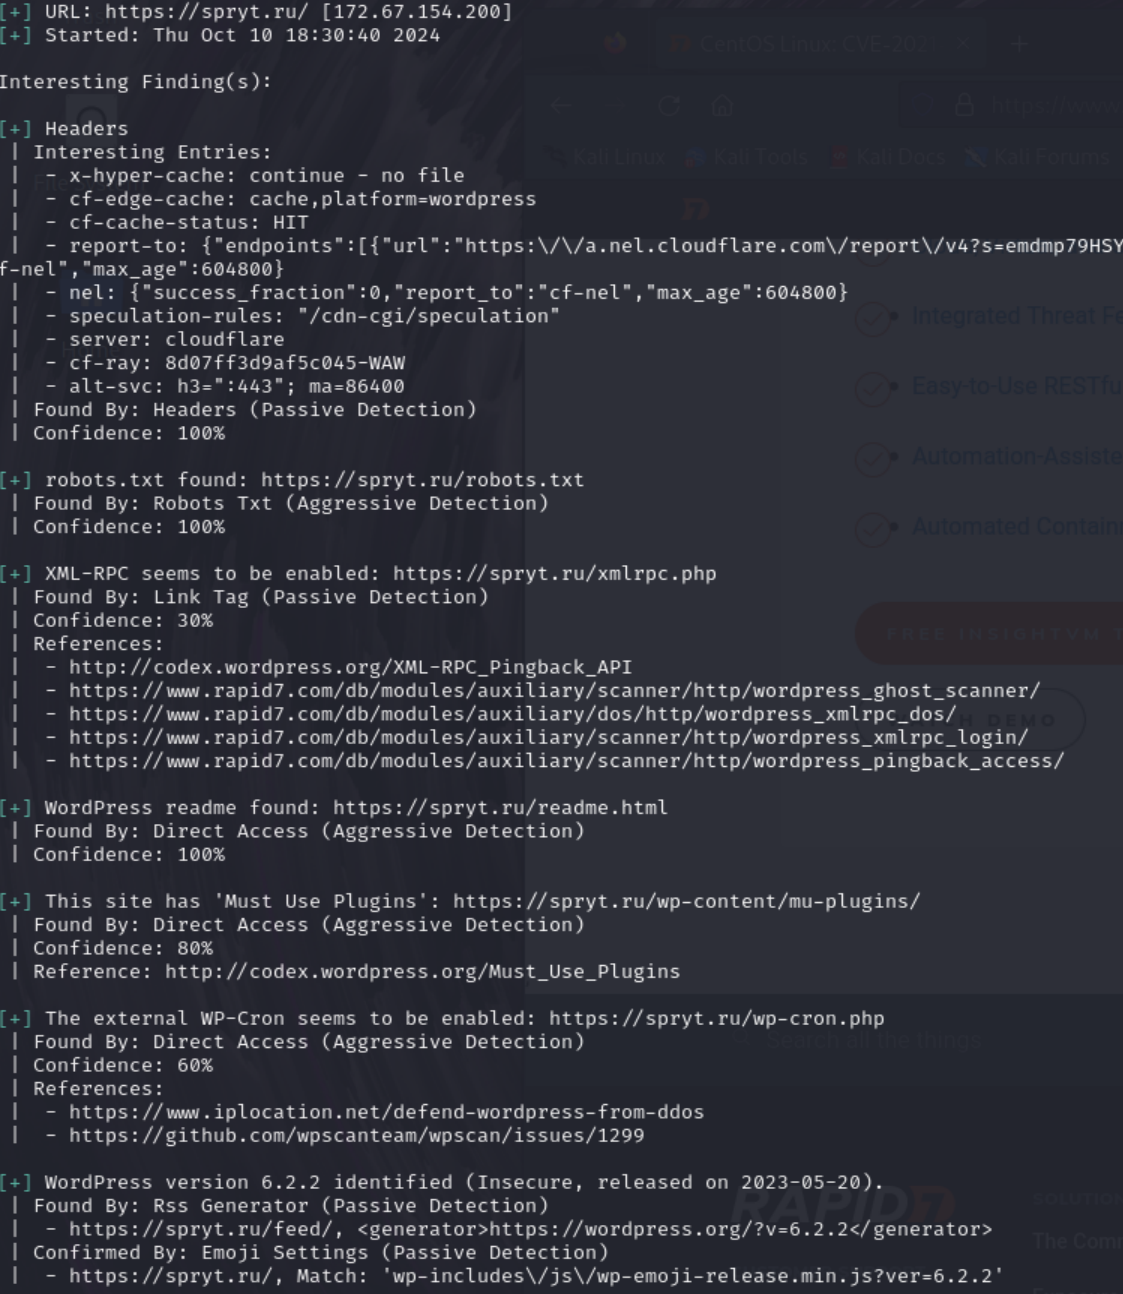
\includegraphics[width=0.7\textwidth]{media/ict/image34}
	\caption*{Рис. 1 - Общее сканирования веб-сервиса}
\end{figure}

\begin{figure}[H]
	\centering
	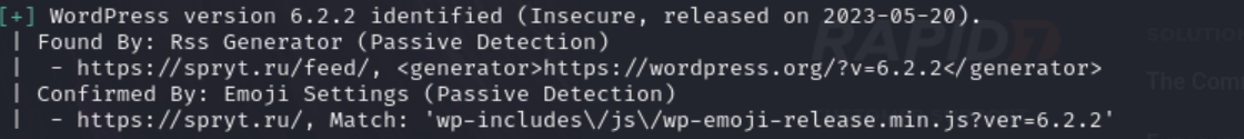
\includegraphics[width=0.8\textwidth]{media/ict/image35}
	\caption*{Рис. 2 - Идентифицированная версия WordPress}
\end{figure}

\begin{figure}[H]
	\centering
	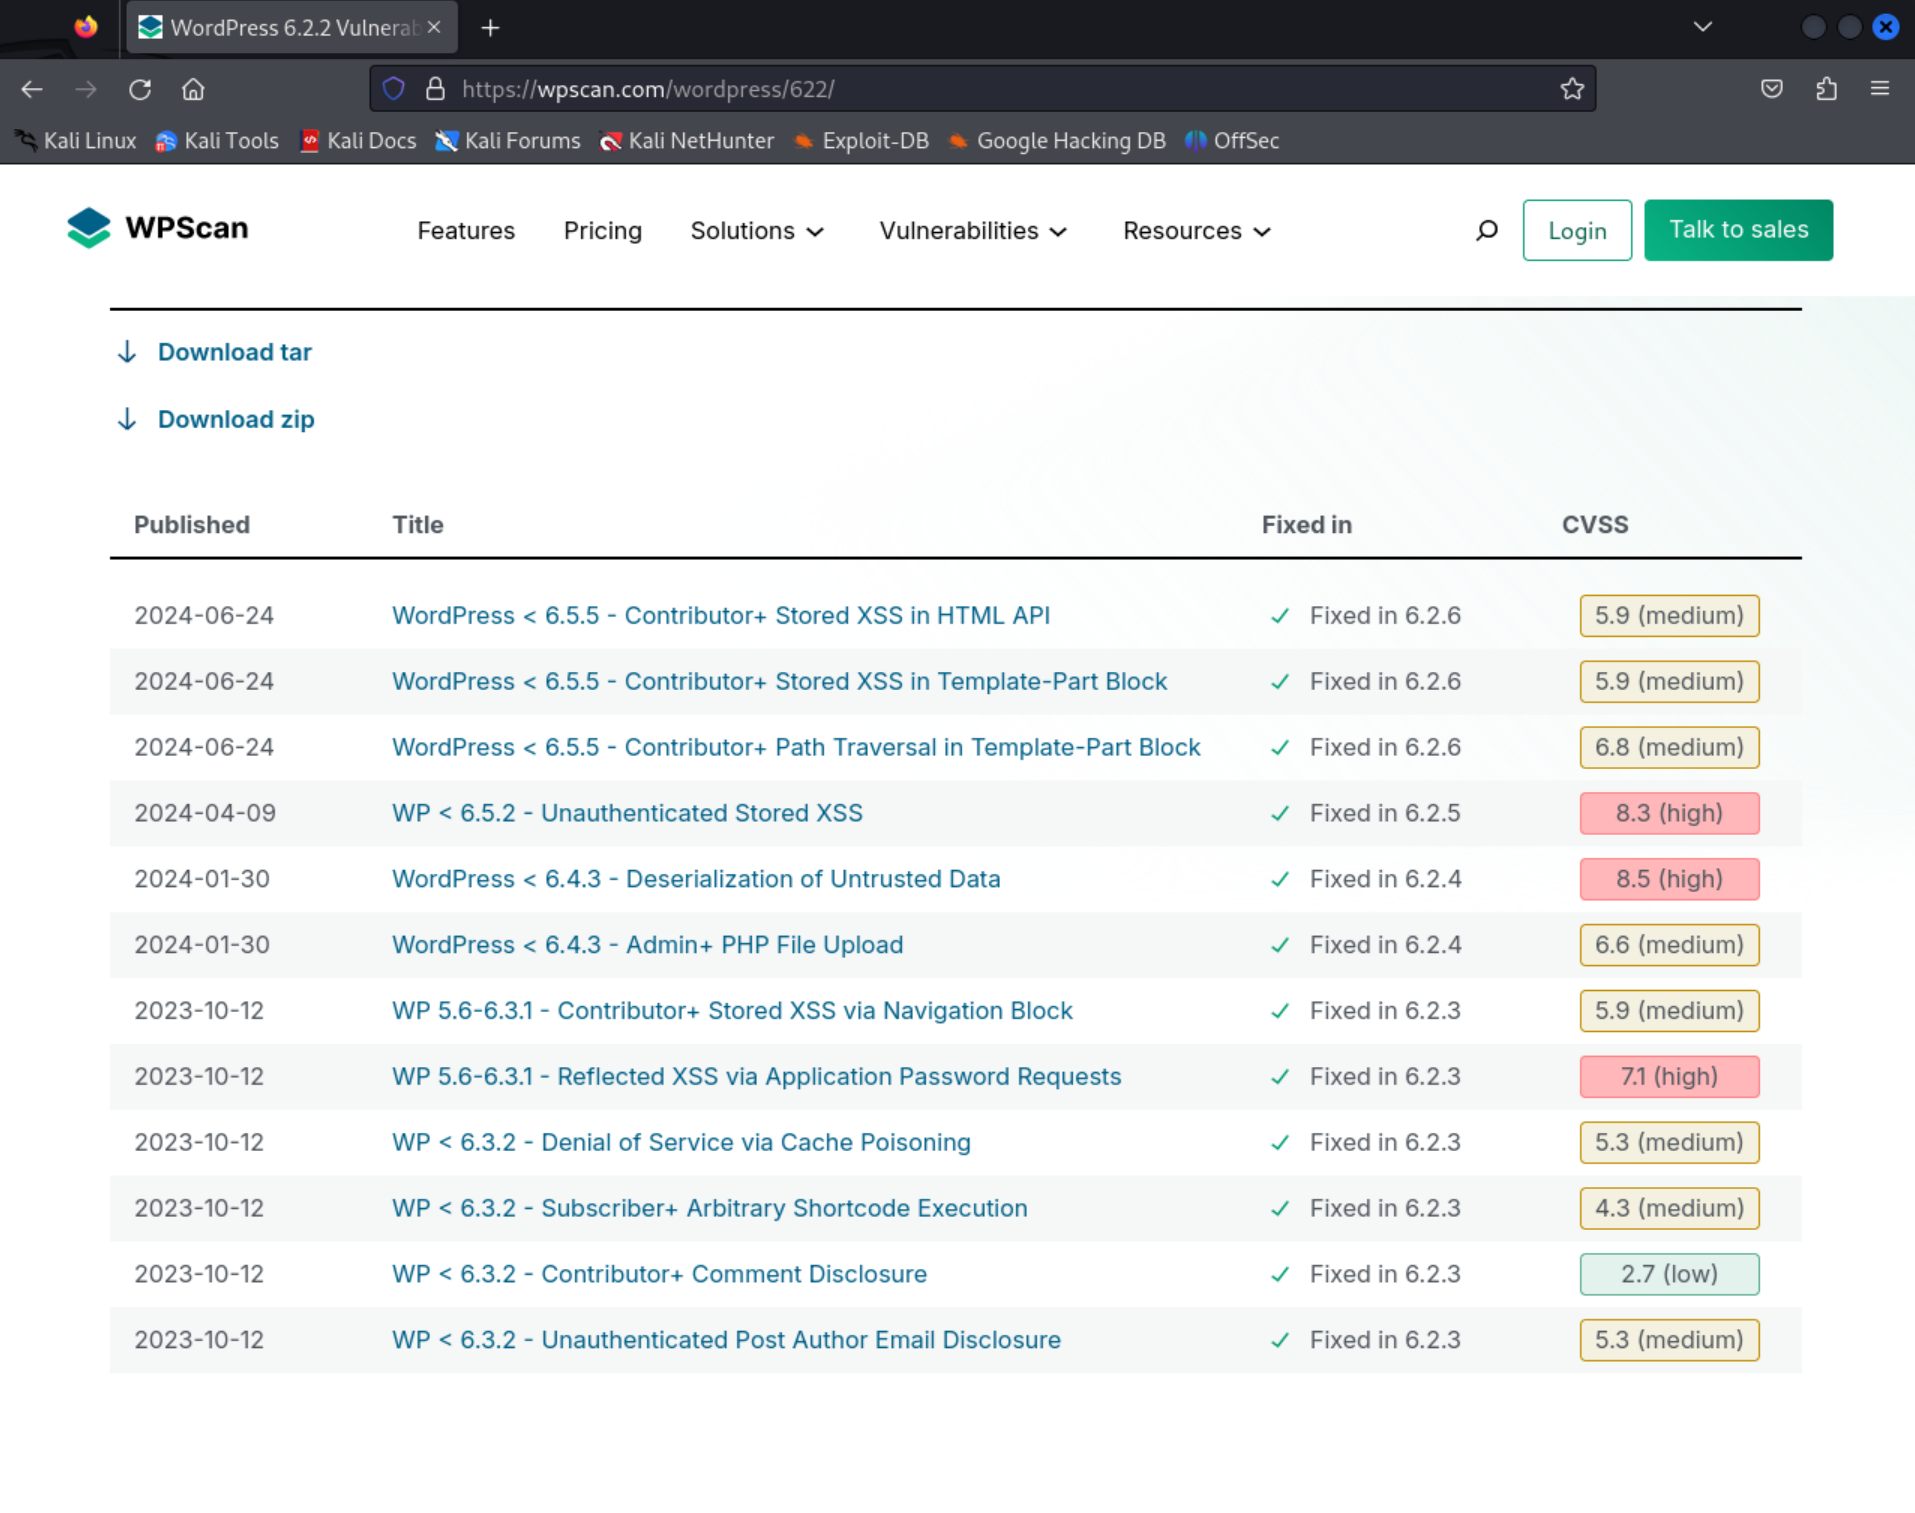
\includegraphics[width=0.8\textwidth]{media/ict/image36}
	\caption*{Рис. 3 - Список эксплойтов}
\end{figure}

\begin{multicols}{2}
Как видим из этого списка с самого сайта инструмента (рисунок 4), уже
есть уязвимости версий 6.2.2 и выше, которые можно использовать в своих
целях. Данный список предоставляет все уязвимости и уровень их опасности
внутри самого веб-сайта. В дальнейшем можно использовать эксплойт XSS
уязвимостей для получения доступа в саму эко систему веб-сайта.
\end{multicols}

\begin{figure}[H]
	\centering
	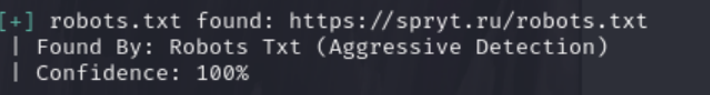
\includegraphics[width=0.7\textwidth]{media/ict/image37}
	\caption*{Рис. 4 - Корневой файл системы}
\end{figure}

\begin{multicols}{2}
Для безопасности сайта лучше скрыть или удалить robots.txt, так как он
содержит данные, которые сможет использовать в своих целях злоумышленник
(рисунок 5).
\end{multicols}

\begin{figure}[H]
	\centering
	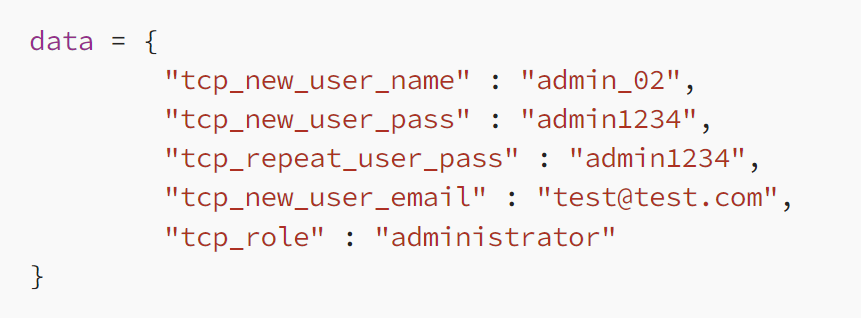
\includegraphics[width=0.7\textwidth]{media/ict/image38}
	\caption*{Рис. 5 - Содержание файла robots.txt}
\end{figure}

Рассмотрим наиболее уязвимости в плагинах и темах веб-сайта (рисунок 6).

\begin{figure}[H]
	\centering
	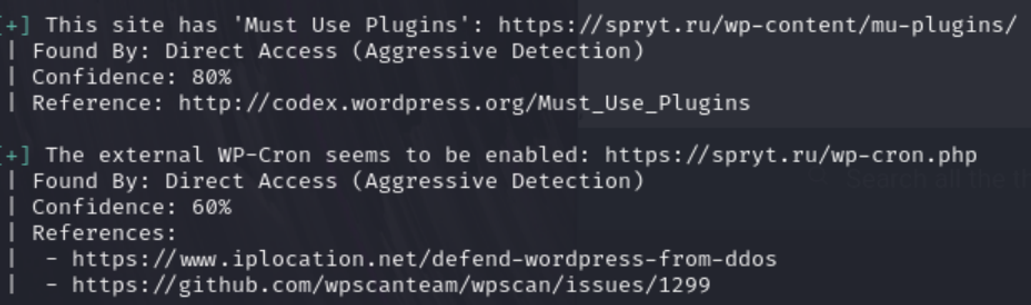
\includegraphics[width=0.7\textwidth]{media/ict/image39}
	\caption*{Рис. 6 - Обнаружение используемого плагина на этом веб-сервисе}
\end{figure}

\begin{multicols}{2}
Используемый данный плагин Must\_use\_plugin не содержит уязвимости, и
он поддерживается самой команды Wpsscan для обеспечения общей
безопасности. В данной работе был преодолён путь с самого верхнего слоя
уязвимостей сайтов до самых нижних, которые могут использовать
злоумышленники.

{\bfseries Выводы.} Учитывая рост интернета, количество веб-приложений,
пользователей и неопытных разработчиков, проблема безопасности
веб-приложений остается актуальной на всех уровнях и требует
комплексного подхода.

В процессе научных исследований проанализирован мощный инструмент
сканирования веб-сервисов Wpscan. Используя его, и благодаря данной
методике анализа уязвимостей администраторы могут вовремя обнаружить и
устранить слабые места в системе безопасности, что позволяет защитить
сайты от распространенных угроз, таких как атаки на устаревшие плагины
или попытки брутфорс.

Были рассмотрены примеры реальных уязвимостей в плагинах и темах
WordPress, что особенно важно для крупных веб-ресурсов, использующих
множество внешних модулей. Данные примеры показывают, как важны
регулярные обновления и мониторинг безопасности для предотвращения
угроз.

В данной работе был исследован сайт Sprut.ru на безопасность. Также были
разработаны рекомендации для улучшения безопасности сайта. В частности,
необходимо обновить версию ядра, убрать или скрыть файл в корневом
каталоге, регулярно проверять веб-ресурс на отсутствие эксплойтов.

Данные мероприятия приводят к выводу о необходимости создания полных
комплексов поиска уязвимостей и нарушений безопасности.
\end{multicols}

\begin{center}
{\bfseries Литература}
\end{center}

\begin{references}
1. Mouratidis, H., Jürjens, J. and Fox, J. Towards a Comprehensive
Framework for Secure Systems \\Development //Advanced Information Systems
Engineering. Springer, Berlin Heidelberg.- 2006.- P. 48-62. DOI
10.1007/11767138\_5

2. Кибератаки//
\href{\%20https://www.tadviser.ru/index.php/Статья:Кибератаки.}{https://www.tadviser.ru/index.php/Статья:Кибератаки.}Дата
обращения :03.11.2024г.

3. Семенов Ю.А. Обзор уязвимостей, некоторых видов атак и средств защиты
{[}Электронный ресурс{]}: // \href{http://book.itep.ru/6/intrusion.htm}{http://book.itep.ru}.-
Дата обращения: 10.11.2024г.

4. Сюткина В. Промышленные предприятия уязвимы для атак, 2018 //
\href{https://www.comnews.ru/content/112938/2018-05-07/promyshlennye-predpriyatiya-uyazvimy-dlya-atak}{https://www.comnews.ru}.
Дата обращения: 19.10.2024г.

5. Zhen Ling, Junzhou Luo, Yiling Xu, Chao Gao, Kui Wu, and Xinwen Fu.
Security Vulnerabilities of Internet of Things: A Case Study of the
Smart Plug System. IEEE Internet of Things Journal.- 2017. -Vol. 4(6) --
P.1899-1909. DOI
\href{https://doi.org/10.1109/JIOT.2017.2707465}{10.1109/JIOT.2017.2707465}

6. Уязвимости корпоративных информационных систем, 2019 /0 \href{https://www.ptsecurity.com/ru-ru/research/analytics/corporate-vulnerabilities-2019}{https://www.ptsecurity.com}
Дата обращения:16.10.2024г.

7. Актуальные киберугрозы: III квартал 2023 года
//\href{https://www.ptsecurity.com/ru-ru/research/analytics/cybersecurity-threatscape-2023-q3}{https://www.ptsecurity.com}.
Дата обращения: \\19.10.2024г.

8. Chaudhry N., Yousaf M.M., Khan M.T. Security assessment of data
management systems for cyber physical system applications //J. Softw
Evol Proc.- 2020.-Vol.32. - P.e2241-1-е2241-9.
\\\href{https://doi.org/10.1002/smr.2241}{DOI 10.1002/smr.2241}

9. Fink G.A., Edgar T.W., Rice T.R. et al. Overview of Security and
Privacy in Cyber‐Physical Systems // In book: Security and Privacy in
Cyber‐Physical Systems. - Makkah, KSA, 2017. - Р. 327-351
\end{references}

\begin{center}
{\bfseries References}
\end{center}

\begin{references}
1. Mouratidis, H., Jürjens, J. and Fox, J. Towards a Comprehensive
Framework for Secure Systems \\Development //Advanced Information Systems
Engineering. Springer, Berlin Heidelberg.- 2006.- pp. 48-62. DOI
10.1007/11767138\_5

2. Kiberataki//\href{https://www.tadviser.ru/index.php/Stat'ja:Kiberataki}{https://www.tadviser.ru}.Data obrashhenija:

03.11.2024g.{[}in Russian{]}

3. Semenov Ju.A. Obzor ujazvimostej, nekotoryh vidov atak i sredstv
zashhity {[}Jelektronnyj resurs{]}: //
http://book.itep.ru/6/intrusion.htm.- Data obrashhenija: 10.11.2024g.
.{[}in Russian{]}

4. Sjutkina V. Promyshlennye predprijatija ujazvimy dlja atak, 2018 //
\href{https://www.comnews.ru/content/112938/2018-05-07/promyshlennye-predpriyatiya-uyazvimy-dlya-atak}{https://www.comnews.ru}.
Data obrashhenija: - 19.10.2024g. {[}in Russian{]}

5. Zhen Ling, Junzhou Luo, Yiling Xu, Chao Gao, Kui Wu, and Xinwen Fu.
Security Vulnerabilities of Internet of Things: A Case Study of the
Smart Plug System. IEEE Internet of Things Journal.- 2017. -Vol. 4(6)
-P.1899-1909. DOI
\href{https://doi.org/10.1109/JIOT.2017.2707465}{10.1109/JIOT.2017.2707465}

6. Ujazvimosti korporativnyh informacionnyh sistem, 2019 /0
\href{https://www.ptsecurity.com/ru-ru/research/analytics/corporate-vulnerabilities-2019}{https://www.ptsecurity.com}
Data \\obrashhenija: 16.10.2024g.{[}in Russian{]}

7. Aktual' nye kiberugrozy: III kvartal 2023 goda
//\href{https://www.ptsecurity.com/ru-ru/research/analytics/cybersecurity-threatscape-2023-q3}{https://www.ptsecurity.com}/.
Data obrashhenija: \\19.10.2024g.{[}in Russian{]}

8. Chaudhry N., Yousaf M.M., Khan M.T. Security assessment of data
management systems for cyber physical system applications //J. Softw
Evol Proc.- 2020.-Vol.32. - P.e2241-1-е2241-9.\\
\href{https://doi.org/10.1002/smr.2241}{DOI 10.1002/smr.2241}

9. Fink G.A., Edgar T.W., Rice T.R. et al. Overview of Security and
Privacy in Cyber‐Physical Systems // In book: Security and Privacy in
Cyber‐Physical Systems. - Makkah, KSA, 2017. - Р. 327-351
\end{references}

\begin{authorinfo}
\emph{{\bfseries Сведения об авторах}}

Даненова Г.Т. - кандидат технических наук, доцент, Карагандинский
технический университет им. Абылкаса Сагинова, г. Караганда, Казахстан,
e-mail: \href{mailto:guldan72@mail.ru}{\nolinkurl{guldan72@mail.ru}};

Манат А.Е.- магистрант, Карагандинский технический университет им.
Абылкаса Сагинова, г. Караганда, Казахстан, e-mail:
\href{mailto:azamatm133@gmail.com}{\nolinkurl{azamatm133@gmail.com}};

Ахметжанов Т.Б.- кандидат технических наук, доцент, Карагандинский
технический университет им. Абылкаса Сагинова, г. Караганда, Казахстан,
e-mail: akhmetzhantalgat@gmail.com;

Коккоз М.М. - кандидат педагогических наук, доцент, Карагандинский
технический университет им. Абылкаса Сагинова, г. Караганда, Казахстан,
e-mail: \href{mailto:makhabbat_k@bk.ru}{\nolinkurl{makhabbat\_k@bk.ru}};

Сайлау қызы Ж. - доктор PhD, Карагандинский технический университет им.
Абылкаса Сагинова, г.Караганда, Казахстан, e-mail:
\href{mailto:s_k_zhuldiz@mail.ru}{\nolinkurl{s\_k\_zhuldiz@mail.ru}}

\emph{Information about the authors}

Danenova G.T. - Сandidate of Technical Sciences, Associate Professor,
Karaganda Technical University named by Abylkas Saginov, Karaganda,
Kazakhstan, e-mail:
\href{mailto:guldan72@mail.ru}{\nolinkurl{guldan72@mail.ru}};

Manat A.E. - grad student, Karaganda Technical University named by
Abylkas Saginov, Karaganda, Kazakhstan, e-mail:\\
\href{mailto:azamatm133@gmail.com}{\nolinkurl{azamatm133@gmail.com}};

Akhmetzhanov T.B. - Сandidate of Technical Sciences, Associate
Professor, Karaganda Technical University named by Abylkas Saginov,
Karaganda, Kazakhstan, e-mail:
\href{mailto:akhmetzhantalgat@gmail.com}{\nolinkurl{akhmetzhantalgat@gmail.com}};

Kokkoz M.M. - Сandidate of Pedagogical Sciences, Associate Professor,
Karaganda Technical University named by Abylkas Saginov, Karaganda,
Kazakhstan, e-mail:
\href{mailto:makhabbat_k@bk.ru}{\nolinkurl{makhabbat\_k@bk.ru}};

Sailau kyzy Zh. - Doctor PhD, Associate Professor, Karaganda Technical
University named by Abylkas Saginov, Karaganda, Kazakhstan, e-mail:
\href{mailto:s_k_zhuldiz@mail.ru}{\nolinkurl{s\_k\_zhuldiz@mail.ru}}
\end{authorinfo}
